% =========================================================================
% Secao 6 - Comparacao com INEP e decomposicao
% =========================================================================

\section{Comparação com o INEP e decomposição do gap}
\label{sec:inep}

A Figura~\ref{fig:pnadc_vs_inep} confronta as séries temporais das
três taxas de transição entre anos (promoção, repetência e evasão)
calculadas a partir da PNADC longitudinal com as taxas oficiais do
INEP, para Brasil e por macroetapa, no período 2007--2024. As
linhas sólidas representam o INEP e as linhas tracejadas a PNADC. A
área sombreada destaca o período pandêmico (2020 e 2021), conforme
discutido na Seção~\ref{sec:agregados}.

\begin{figure}[htbp]
\centering
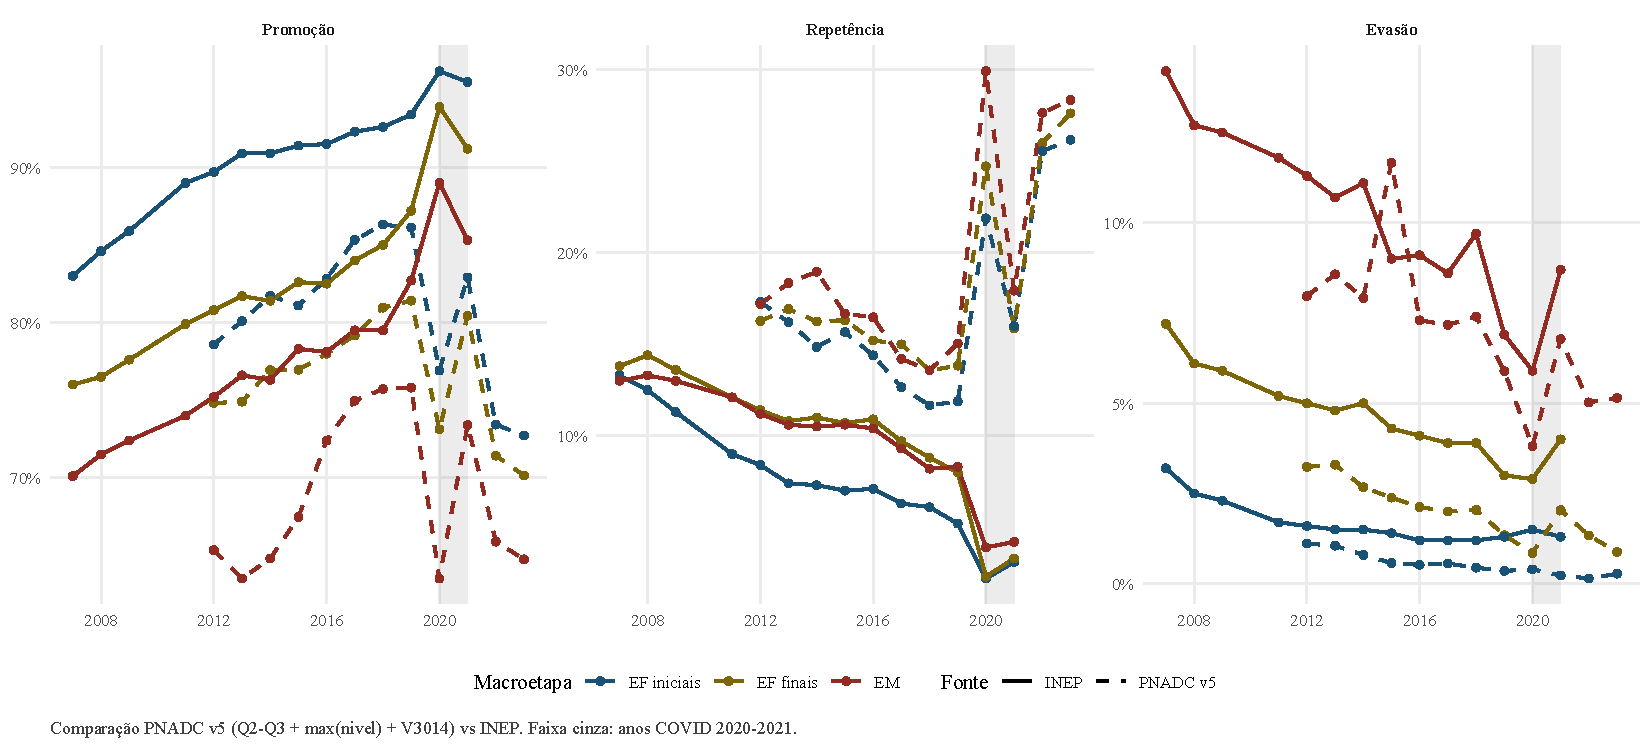
\includegraphics[width=\textwidth]{../DataWork/5_Figures/output/F5_pnadc_vs_inep.pdf}
\caption{PNADC longitudinal vs.\ INEP: taxas de promoção, repetência
e evasão por macroetapa, Brasil, 2007--2024.}
\label{fig:pnadc_vs_inep}
\figurenote{A série INEP Taxa de Transição (linha sólida) cobre o
período 2007--2021 e foi descontinuada após a transição 2021--2022.
A série PNADC longitudinal (linha tracejada) cobre 2012--2024. A
área cinza marca o período COVID-19 (2020 e 2021).}
\end{figure}

Sob a metodologia reformulada da Seção~\ref{ssec:definicoes}, com
referência em $Q_2$ e $Q_3$ e uso de $\max(\text{nível})$ em $t+1$,
a PNADC e o INEP ficam significativamente mais alinhadas no EF, com
gap residual mais visível no EM. A Tabela~\ref{tab:t4_pnadc_inep}
reporta a comparação para a transição 2019/2020.

\begin{table}[htbp]
\centering
\caption{Comparação PNADC vs.\ INEP -- Transição 2019/2020, Brasil}
\label{tab:t4_pnadc_inep}
\begin{threeparttable}
\small
\begin{tabular}{lccccc}
\toprule
                       & \multicolumn{3}{c}{Indicador (\%)} & \multicolumn{2}{c}{Gap} \\
\cmidrule(lr){2-4} \cmidrule(lr){5-6}
                       & Promoção & Repetência & Evasão & PP & Relativo \\
\midrule
\multicolumn{6}{l}{\textit{EF iniciais (Anos Iniciais)}} \\
INEP                   & 93,5 & 5,1 & 1,1  & --   & --    \\
PNADC                  & 76,6 & 22,9 & 0,3 & $-$16,9 & $-$18\% \\
\midrule
\multicolumn{6}{l}{\textit{EF finais (Anos Finais)}} \\
INEP                   & 86,0 & 9,8 & 3,5  & --   & --    \\
PNADC                  & 71,5 & 24,7 & 1,6 & $-$14,5 & $-$17\% \\
\midrule
\multicolumn{6}{l}{\textit{Ensino Médio (Total)}} \\
INEP                   & 82,7 & 8,3 & 6,9  & --   & --    \\
PNADC                  & 49,0 & 17,3 & 24,5 & $-$33,7 & $-$41\% \\
\bottomrule
\end{tabular}
\begin{tablenotes}
\footnotesize
\item \textit{Nota:} Fontes -- INEP Taxa de Transição 2019/2020 (Brasil),
publicada em \citet{INEP_transicao}; PNADC trimestral, painel longitudinal,
transição 2019$\to$2020 medida via primeira observação em $t$ vs.\ primeira
observação em $t+1$. Gap em pontos percentuais (PP) e em \% do nível INEP.
A diferença substancial para o EM reflete principalmente a definição
operacional de promoção: o INEP classifica como promovidos os alunos que
concluíram o 3\textsuperscript{o} EM mesmo sem matrícula subsequente;
nossa metodologia inicial exige frequência escolar em $t+1$. Versão refinada
da PNADC em desenvolvimento.
\end{tablenotes}
\end{threeparttable}
\end{table}


Para o EF iniciais em 2019, o INEP reporta promoção de 93,5\% e
nossa estimativa PNADC é de 85,5\%, gap de 8,0 pontos percentuais.
Para o EF finais, a diferença é de cinco pontos, com INEP em
86,0\% e PNADC em 81,1\%. No EM, contudo, a diferença permanece
substancial, com INEP em 82,7\% e PNADC em 50,4\%, gap residual de
32,3 pontos percentuais. A análise a seguir investiga as fontes
desse gap.

Para cada par (etapa, ano, indicador), a diferença
$\Delta = \text{INEP} - \text{PNADC}$ é decomposta em cinco
fontes,
\[
\Delta = \underbrace{R}_{\text{retorno}}
      + \underbrace{U}_{\text{universo}}
      + \underbrace{S}_{\text{amostragem}}
      + \underbrace{C}_{\text{sub-cobertura}}
      + \underbrace{M}_{\text{medida residual}}.
\]
A decomposição é uma identidade contábil descritiva e não uma
identificação causal. Os componentes $R$, $U$, $S$ e $C$ são
estimáveis diretamente das duas fontes, ao passo que $M$ é
definido por construção como o resíduo,
$M = \Delta - (R + U + S + C)$, e captura quaisquer fontes de
divergência não explicitadas, incluindo erros de classificação,
diferenças entre a semana de referência da PNADC e o ano letivo do
Censo Escolar, e demais discrepâncias metodológicas que não são
$R$, $U$, $S$ ou $C$. Reportamos $M$ explicitamente, em vez de
ocultá-lo em alguma agregação.

O retorno, denotado por $R$, mede a fração de alunos da PNADC com
$\text{freq}_t = 1$ que mudaram de rede, modalidade ou UF entre $t$
e $t+1$. Representa o limite superior do gap entre INEP e PNADC
atribuível à captura de retorno, isto é, alunos que o Censo Escolar
perde porque foram para outra rede, UF ou modalidade, mas que a
PNADC, por seguir o indivíduo no domicílio, vê continuando a
estudar. A Figura~\ref{fig:captura_retorno} reporta o componente
$R$ por subgrupo. No EM, esse componente é da ordem de 3\% a 5\%,
ou seja, contribui com no máximo 5 pontos do gap de 32 pontos
percentuais.

\begin{figure}[htbp]
\centering
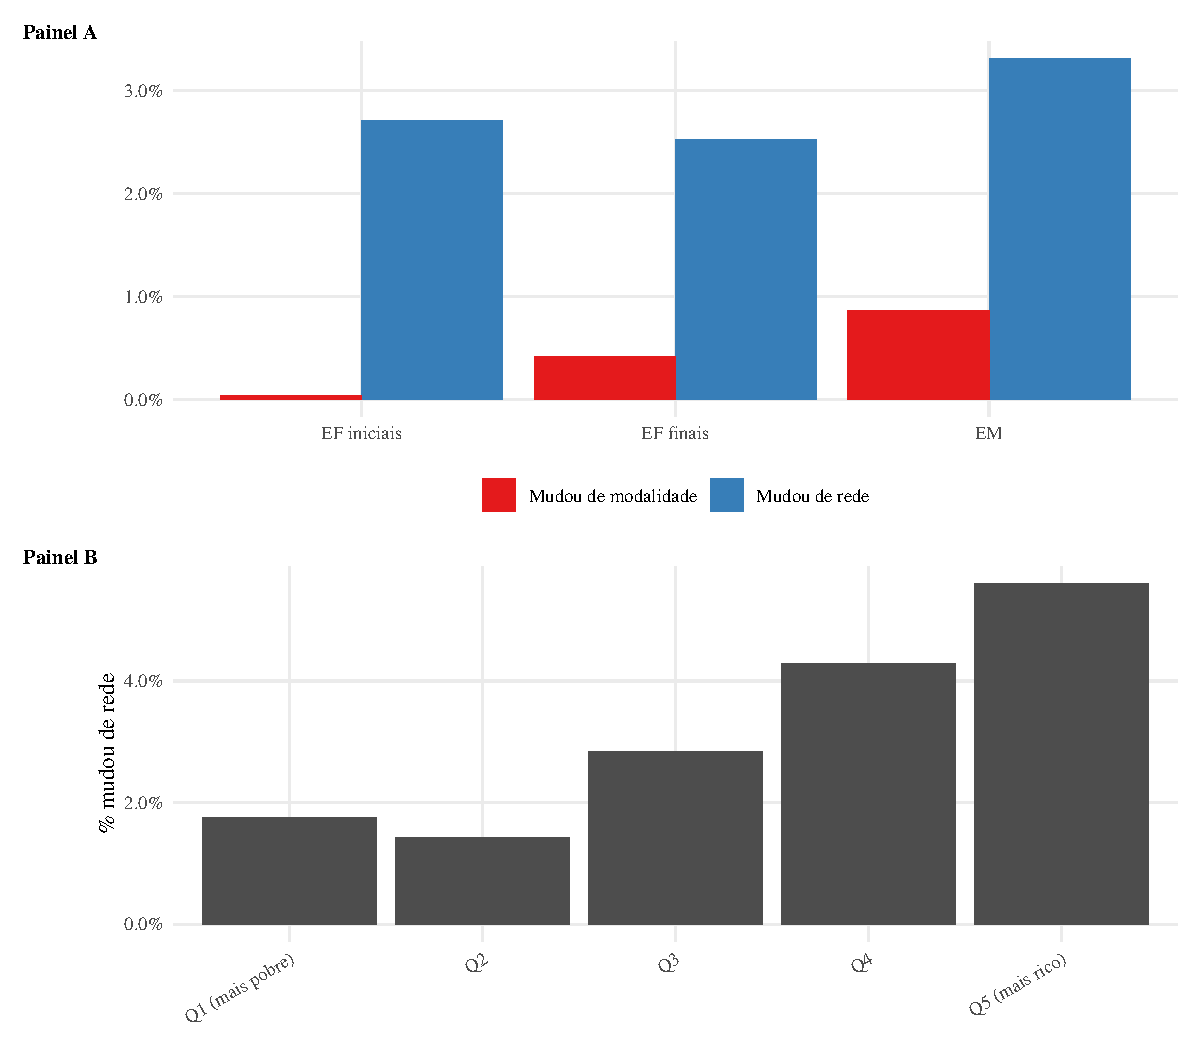
\includegraphics[width=0.95\textwidth]{../DataWork/5_Figures/output/F3_captura_retorno.pdf}
\caption{Captura de retorno por macroetapa e quintil de renda,
PNADC 2018--2023.}
\label{fig:captura_retorno}
\figurenote{Percentual de alunos com \texttt{V3002=1} em $t+1$ que
mudaram de rede ou modalidade entre $t$ e $t+1$.}
\end{figure}

O universo, denotado por $U$, é a diferença entre os denominadores,
isto é, entre a população estudando em $t$ na PNADC, extrapolada
pelo peso, e as matrículas no Censo Escolar de $t$. Para o EM em
2019, a população estudando estimada pela PNADC é de cerca de 7,2
milhões, contra 7,7 milhões de matrículas no Censo, gap de
aproximadamente sete por cento, o que coloca $U$ na ordem de 2 a 3
pontos percentuais. A amostragem, denotada por $S$, corresponde ao
intervalo de confiança de 95\% por \emph{bootstrap} das estimativas
PNADC. Para a promoção do EM em 2019, com $n \approx 5{.}700$, a
semiamplitude é de aproximadamente 1,3 ponto percentual. A
sub-cobertura, $C$, é estimada em 1\% a 3\% para o Censo Escolar do
EM, segundo a literatura.

A soma de $R + U + S + C$ no EM em 2019 fica em torno de 10 pontos
percentuais. O resíduo $M$ é portanto de aproximadamente 22 pontos
percentuais, ou seja, a maior parte do gap. Investigando a fundo,
identifica-se uma fonte definicional dominante. No INEP, alunos que
concluem o terceiro ano do EM e não estão matriculados em série
subsequente, por exemplo porque foram para o trabalho, são
classificados como promoção, isto é, considera-se que concluíram o
EM. Em nossa metodologia operacional, a promoção requer
\texttt{V3002=1} (frequenta escola) e nível de $t+1$ superior ao
nível de $t$. Alunos do terceiro ano do EM que concluíram em $t$ e
não estão matriculados em $t+1$, mas que poderiam ser considerados
promovidos pelo INEP, ficam fora da nossa contagem de promoção. Em
2019, aproximadamente 22\% dos alunos no terceiro ano do EM no
painel apresentam essa situação, ou seja, \texttt{V3002=2} em $t+1$
com curso anterior reportado em \texttt{V3013A} como ``ensino médio
completo''. Esses 22\% explicariam, portanto, a maior parte do
componente $M$ no EM.

Uma versão refinada da PNADC ajustaria a definição de promoção para
incluir esses casos, identificando a conclusão do EM via
\texttt{V3013A} e \texttt{VD3004}. Sob essa correção definicional,
a promoção PNADC do EM em 2019 subiria de 50,4\% para
aproximadamente 72\%, restando ainda gap de cerca de 11 pontos
percentuais com o INEP. Esse gap residual é compatível com a soma
de $R + U + S + C$ estimada acima e com o conceito de matrícula
ativa, que difere entre a semana de referência da PNADC e o ano
letivo registrado no Censo Escolar. Implementar essa correção
definicional é deixado para uma versão futura do trabalho, sendo
relativamente direto na infraestrutura de código disponível. A
interpretação substantiva, contudo, importa. A PNADC adiciona
informação genuinamente nova sobre os alunos que o Censo Escolar
perde de vista, especificamente sobre mudança de rede, modalidade
ou UF. Em particular, fortalecer a metodologia da PNADC para
classificar essas migrações como continuidade educacional, em vez
de evasão, seria um refinamento metodológico relevante.
